% !TEX root = main.tex
\section{Setup}
\label{sec:Aufbau}
This chapter is about the setup and execution process of this experiment. To understand which part of the experiment has what use, it is necessary to have a look at the components of the setup.\newline
Figure \ref{fig:Aufbau} shows the different coils which are necessary for the EFNMR measurement. The innerst coil B$_1$ coil is the excite and collect coil which is described in the previous chapter. The outer coil is to prepolarize the sample. This is necessary to obtain a stronger signal. By applying a strong magnetic field orthogonal to the earths magnetic field the spins align in the direction of the prepolarizing pulse and provides a bulk polarized nuclear magnetization across the sample. The middle coil is the gradient coil. This coil erases the inhomogenious magnetic field which always occurs for different uncertainty reasons. This coil is also used for the 2D imaging of the probe by adjusting the components of the magnetic field. Via the computer program \textit{Prospa} and the spectrometer the currents of the coil can be adjust and the induced signals can be measured.
\begin{figure}[H]
    \centering
    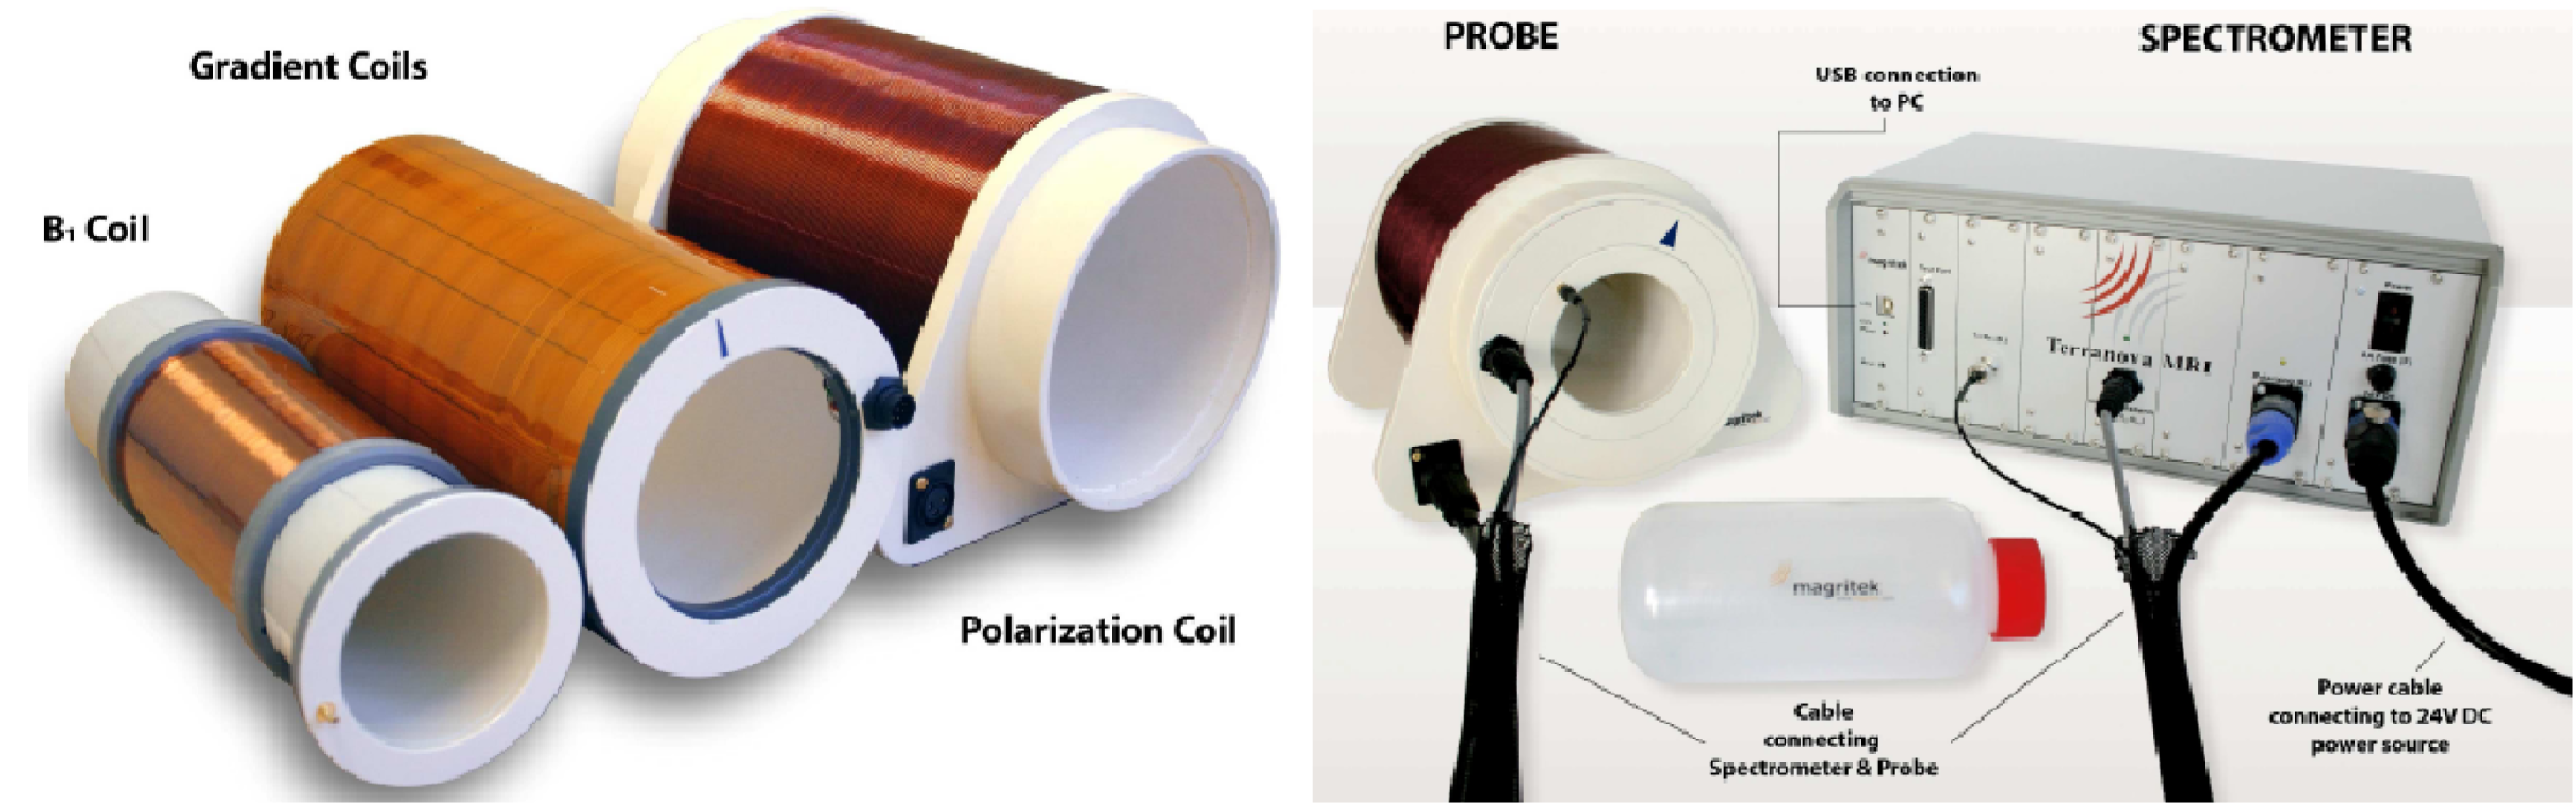
\includegraphics[width= \textwidth]{Aufbau.png}   
    \caption[Setup of the \textit{Terranova-MRI EFNMR}. \cite{Bild}]{Setup of the \textit{Terranova-MRI EFNMR}. On the left handside the coils B$_1$ (excite and collect coil), gradient coil (homogenious magnetic field and 2D scanning coil) and the prepolarizing coil B$_p$ are seen. The right hand side shows the water sample which has been used and the spectrometer which adjusts the right signals to the coils. \cite{Bild}}
    \label{fig:Aufbau}
\end{figure}
